\chapter{Основные теоретические сведения}
RISC-V является открытым современным набором команд, который может использоваться для построения как микроконтроллеров, так и высокопроизводительных микропроцессоров. Таким образом, термин RISC-V фактически является названием для семейства различных систем команд, которые строятся вокруг базового набора команд, путем внесения в него различных расширений.

В данной работе исследуется набор команд RV32I, который включает в себя основные команды 32-битной целочисленной арифметики кроме умножения и деления. 

\section{Модель памяти}
Архитектура RV32I предполагает плоское линейное 32-х битное адресное пространство. Минимальной адресуемой единицей информации является 1 байт. Используется порядок байтов от младшего к старшему (Little Endian), то есть, младший байт 32-х битного слова находится по младшему адресу (по смещению 0). Отсутствует разделение на адресные пространства команд, данных и ввода-вывода. Распределение областей памяти между различными устройствами (ОЗУ, ПЗУ, устройства ввода-вывода) определяется реализацией.

\section{Система команд}
Большая часть команд RV32I является трехадресными, выполняющими операции над двумя заданными явно операндами, и сохраняющими результат в регистре. Операндами могут являться регистры или константы, явно заданные в коде команды. Операнды всех команд задаются явно. 

Архитектура RV32I, как и большая часть RISC-архитектур, предполагает разделение команд на команды доступа к памяти (чтение данных из памяти в регистр или запись данных из регистра в память) и команды обработки данных в регистрах.

\chapter{Общая программа}

Рассмотрим пример небольшой программы для RV32I, которым мы будем пользоваться далее
для исследования процесса выполнения команд.

Данная программа выполняет суммирование значений элементов масcива слов и увеличивает
это значение на 1 - Листинг \ref{lst:v1}.
\begin{lstlisting}[label=lst:v1,caption=Пример программы]
    .section .text (1)
	.globl _start; (2)
	len = 8 #Размер массива (3)
	enroll = 4 #Количество обрабатываемых элементов за одну итерацию
	elem_sz = 4 #Размер одного элемента массива
_start: (4)
	addi x20, x0, len/enroll (5)
	la x1, _x (6)
	loop:
	lw x2, 0(x1) (7)
	add x31, x31, x2 (8)
	lw x2, 4(x1)
	add x31, x31, x2
	lw x2, 8(x1)
	add x31, x31, x2
	lw x2, 12(x1)
	add x31, x31, x2
	addi x1, x1, elem_sz*enroll (9)
	addi x20, x20, -1 (10)
	bne x20, x0, loop (11)
	addi x31, x31, 1
forever: j forever (12)

.section .data (13)
_x: .4byte 0x1 (14)
	.4byte 0x2
	.4byte 0x3
	.4byte 0x4
	.4byte 0x5
	.4byte 0x6
	.4byte 0x7
	.4byte 0x8
\end{lstlisting}

\clearpage

\begin{enumerate}
	\item Объявление секции $.text$, содержащей исполняемый код.
	\item Объявление символа $\_start$, имеющего глобальную видимость. Символ $\_start$ это специальный символ, обозначающий точку входа в программу.
	\item Метка.
	\item Объявление констант.
	\item Арифметические выражения над константами могут использоваться в командах
	на месте непосредственного операнда.
	\item Загрузка в $x1$ адреса символа $\_x$ (то есть, начала массива).
	\item Загрузка в $x2$ числа по адресу, содержащемуся в $x1$ по смещению 0.
	\item Добавление к $x31$ (который хранит результат) значения $x2$.
	\item Смещение указателя $x1$.
	\item Уменьшение счетчика цикла.
	\item Условный переход на метку $loop$.
	\item Бесконечный цикл.
	\item Объявление секции данных.
	\item Начало описания массива.
\end{enumerate}

\clearpage

Дизассемблерный код представлен на листинге \ref{lst:v2}.

\begin{lstlisting}[label=lst:v2,caption=Дизассемблированный код примера программы]
Disassembly of section .text:

80000000 <_start>:
80000000:       00200a13        addi    x20,x0,2
80000004:       00000097        auipc   x1,0x0
80000008:       03c08093        addi    x1,x1,60 # 80000040 <_x>

8000000c <lp>:
8000000c:       0000a103        lw      x2,0(x1)
80000010:       002f8fb3        add     x31,x31,x2
80000014:       0040a183        lw      x3,4(x1)
80000018:       003f8fb3        add     x31,x31,x3
8000001c:       0080a203        lw      x4,8(x1)
80000020:       00c0a283        lw      x5,12(x1)
80000024:       004f8fb3        add     x31,x31,x4
80000028:       005f8fb3        add     x31,x31,x5
8000002c:       01008093        addi    x1,x1,16
80000030:       fffa0a13        addi    x20,x20,-1
80000034:       fc0a1ce3        bne     x20,x0,8000000c <lp>
80000038:       001f8f93        addi    x31,x31,1

8000003c <lp2>:
8000003c:       0000006f        jal     x0,8000003c <lp2>
\end{lstlisting}

\clearpage

Можно сказать, что данная программа эквивалентна следующему псевдокоду на языке C, представленному на листинге \ref{lst:v3}.

\begin{lstlisting}[label=lst:v3,caption=Псевдокод общей программы]
#define len 8
#define enroll 4
#define elem_sz 4
int _x[]={1,2,3,4,5,6,7,8};
void _start() {
	int x20 = len/enroll;
	int *x1 = _x;
	
	do {
		int x2 = x1[0];
		x31 += x2;
		x2 = x1[1];
		x31 += x2;
		x2 = x1[2];
		x31 += x2;
		x2 = x1[3];
		x31 += x2;
		x1 += enroll;
		x20--;
	} while(x20 != 0);
	x31++;
	while(1){}
}
\end{lstlisting}

\chapter{Результаты исследования программы}
Задания выполнялись по варианту 9.

\section{Задание №1}

\subsection*{Условие задания}

В процесссе выполнения задания необходимо выполнить следующие действия:
\begin{enumerate}
	\item Ознакомиться с теоретической частью, внимательно изучить примеры.
	\item Перейти в подкаталог $src$ командой $cd$ $riscv-lab/src$.
	\item Выполнить сборку, запустив команду $gmake$. Убедиться, что был создан файл $test.hex$, содержащий шестнадцатеричное представление программы, а в окне терминала отобразился дизассемблерный листинг. Сравнить дизассемблерный листинг с тем, который приведен в примере.
	\item Создать новый файл, содержащий текст программы по индивидуальному варианту (см. Индивидуальные варианты). Поместить его в каталог $src$. Текст программы сохранить в файле с расширением $.s$.
	\item Изучить текст программы по индивидуальному варианту. Поместить в отчете псевдокод, соответствующий данной программе.
	\item Анализируя исходный текст программы, ответьте на вопрос: какое значение должно содержаться в регистре $x31$ в конце выполнения программы?
	\item Изменить в $Makefile$ строку $SRC=$ так, чтобы ее содержимое соответствовало имени файла с текстом программы без расширения .s.
	\item Выполнить компиляцию командой $gmake$. В процессе будет создан файл с расширением $.hex$, хранящий содержимое памяти команд и данных, а в окне терминала отобразится дизассемблерный листинг, который необходимо поместить в отчет вместе с исходным текстом.
\end{enumerate}

\subsection*{Результаты выполнения}

\begin{lstlisting}[label=lst:v11,caption=Код программы 9 варианта]
	.section .text
	.globl _start;
	len = 8 
	enroll = 4
	elem_sz = 4 
	
_start:
	addi x20, x0, len/enroll
	la x1, _x
	lp:
	lw x2, 0(x1)
	add x31, x31, x2 #!
	lw x3, 4(x1)
	add x31, x31, x3
	lw x4, 8(x1)
	lw x5, 12(x1)
	add x31, x31, x4
	add x31, x31, x5
	addi x1, x1, elem_sz*enroll
	addi x20, x20, -1
	bne x20, x0, lp
	addi x31, x31, 1
lp2: j lp2
	
	.section .data
_x: .4byte 0x1
	.4byte 0x2
	.4byte 0x3
	.4byte 0x4
	.4byte 0x5
	.4byte 0x6
	.4byte 0x7
	.4byte 0x8
\end{lstlisting}

Выполнение команды $gmake$, после присвоения $SRC=$ название файла, где содержится код программы варианта 9, в мое случае этот файл был назван $lab\_02\_09$, это показано на рисунке \ref{img:t1-gamake}

\begin{figure}[h]
	\centering
	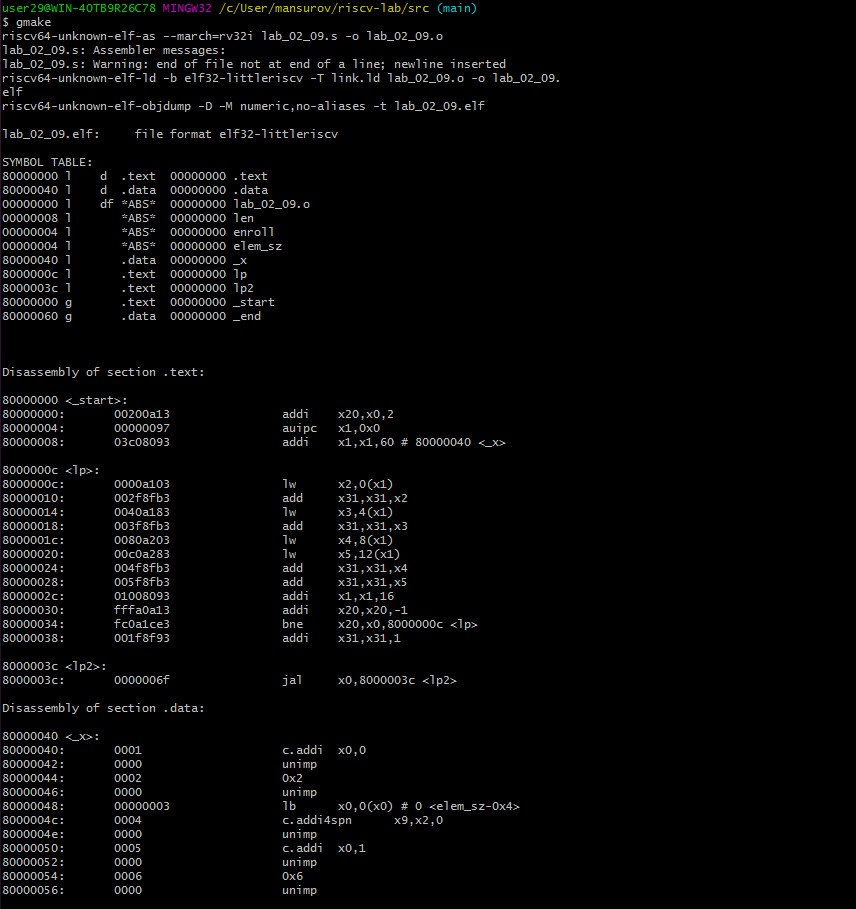
\includegraphics[height=0.8\textheight]{img/t1-gmake.jpg}
	\caption{Скриншот запуска gmake для программы по варианту 9}
	\label{img:t1-gamake}
\end{figure}

\clearpage

\begin{lstlisting}[label=lst:v22,caption=Дизассемблированный код 9 варианта]
Disassembly of section .text:

80000000 <_start>:
80000000:       00200a13        addi    x20,x0,2
80000004:       00000097        auipc   x1,0x0
80000008:       03c08093        addi    x1,x1,60 # 80000040 <_x>

8000000c <lp>:
8000000c:       0000a103        lw      x2,0(x1)
80000010:       0040a183        add     x31,x31,x2
80000014:       0080a203        lw      x4,8(x1)
80000018:       00c0a283        add     x31,x31,x3
8000001c:       002f8fb3        lw      x3,4(x1)
80000020:       003f8fb3        add     x31,x31,x4
80000024:       004f8fb3        lw      x5,12(x1)
80000028:       005f8fb3        add     x31,x31,x5
8000002c:       01008093        addi    x1,x1,16
80000030:       fffa0a13        addi    x20,x20,-1
80000034:       fc0a1ce3        bne     x20,x0,8000000c <lp>
80000038:       001f8f93        addi    x31,x31,1

8000003c <lp2>:
8000003c:       0000006f        jal     x0,8000003c <lp2>
\end{lstlisting}

\clearpage
Можно сказать, что данная программа эквивалентна следующему псевдокоду на языке C, представленному на листинге \ref{lst:v33}.

\begin{lstlisting}[label=lst:v33,caption=Псевдокод программы 9 варианта]
#define len 8
#define enroll 4
#define elem_sz 4
int _x[]={1,2,3,4,5,6,7,8};
void _start() {
	int x20 = len/enroll;
	int *x1 = _x;
	
	do {
		int x2 = x1[0];
		x31 += x2;
		int x3 = x1[1];
		x31 += x3;
		int x4 = x1[2];
		x31 += x4;
		int x5 = x1[3];
		x31 += x5;
		x1 += enroll;
		x20--;
	} while(x20 != 0);
	x31++;
	while(1){}
}
\end{lstlisting}

После выполнения программы по варианту 9 в $x31$ будет записано \newline число 38 (подсчитано вручную и написанной программы на языке С по псевдокоду).

\clearpage

\section{Задание №2}

\subsection*{Условие задания}
В ходе выполнения данного задания необходимо выполнить следующие действия:
\begin{enumerate}
	\item Открыть проект $riscv-lab/taiga/taiga.qpf$ в среде $Intel$ $Quartus$. При запуске $Intel$ $Quartus$, если потребуется, выбрать опцию $Run$ $the$ $Quartus$ $Prime$ $software$.
	\item Выполнить синтез проекта выбрав пункт меню Processing → Start → Start Analysis \& Synthesis.
	\item Запустить симуляцию в среде Modelsim. Для этого выбрать в меню Quartus пункт Tools → Run Simulation Tool → RTL Simulation.
	\item Запустить симуляцию, набрав в командной строке Modelsim команду $run$ $460us$.
	\item Изучить список сигналов, приведенных в окне Wave.
	\item Получить снимок экрана, содержащий временную диаграмму выполнения стадий выборки и диспетчеризации команды с адресом 8000002с на первой итерации.
\end{enumerate}

\clearpage

\subsection*{Результаты выполнения}

После выполнения пунктов 1-4 запускается симуляция в среде Modelsim, как видно на рисунке \ref{img:modelsim}.

\begin{figure}[h]
	\centering
	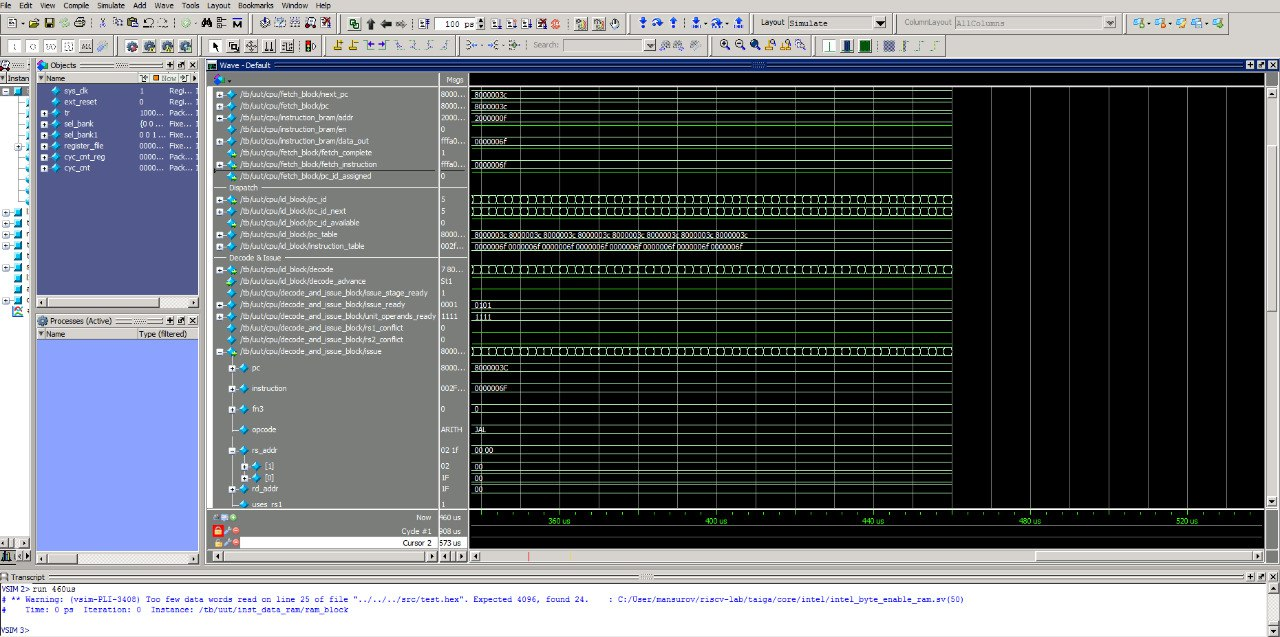
\includegraphics[height=0.33\textheight]{img/sim-modelsim.jpg}
	\caption{Скриншот запуска симуляция в среде Modelsim}
	\label{img:modelsim}
\end{figure}

\clearpage

На рисунке \ref{img:t2-modelsim} снимок экране симуляции в среде Modelsim на стадии выборки и диспетчеризации  команды с адресом 8000002с на первой итерации.

\begin{figure}[h]
	\centering
	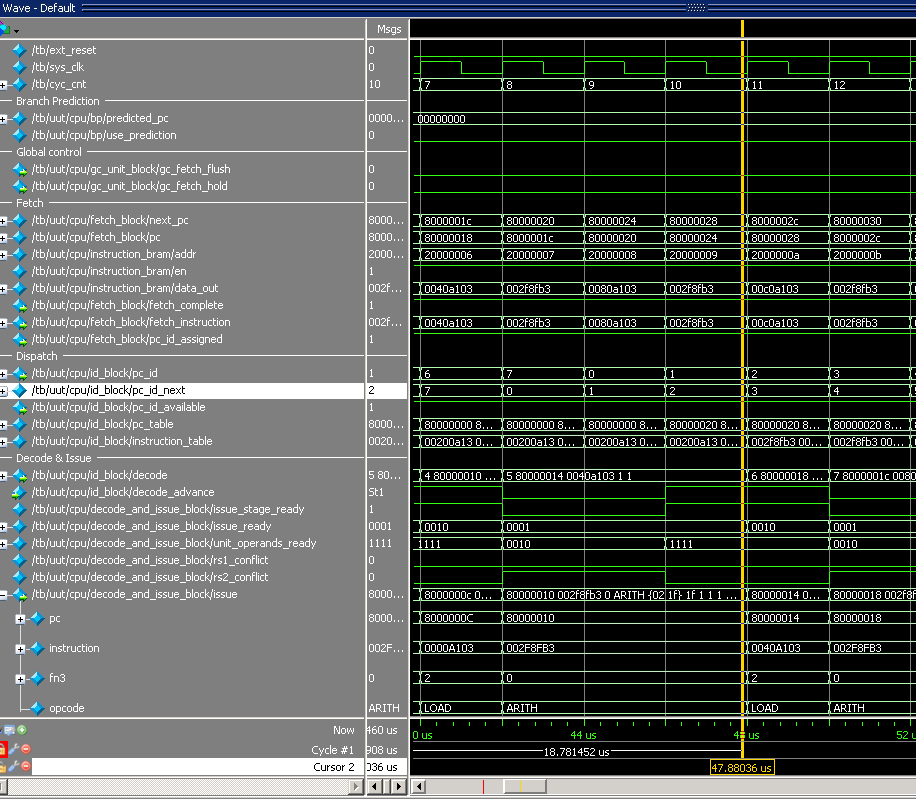
\includegraphics[height=0.57\textheight]{img/t2-modelsim}
	\caption{Скриншот запуска симуляция в среде Modelsim -- команды с адресом 8000002с на первой итерации.}
	\label{img:t2-modelsim}
\end{figure}

\clearpage

\section{Задание №3}

\subsection*{Условие задания}
Получить снимок экрана, содержащий временную диаграмму выполнения стадии декодирования и планирования на выполнение команды с адресом 8000000с на второй итерации.

\subsection*{Результаты выполнения}

\begin{figure}[h]
	\centering
	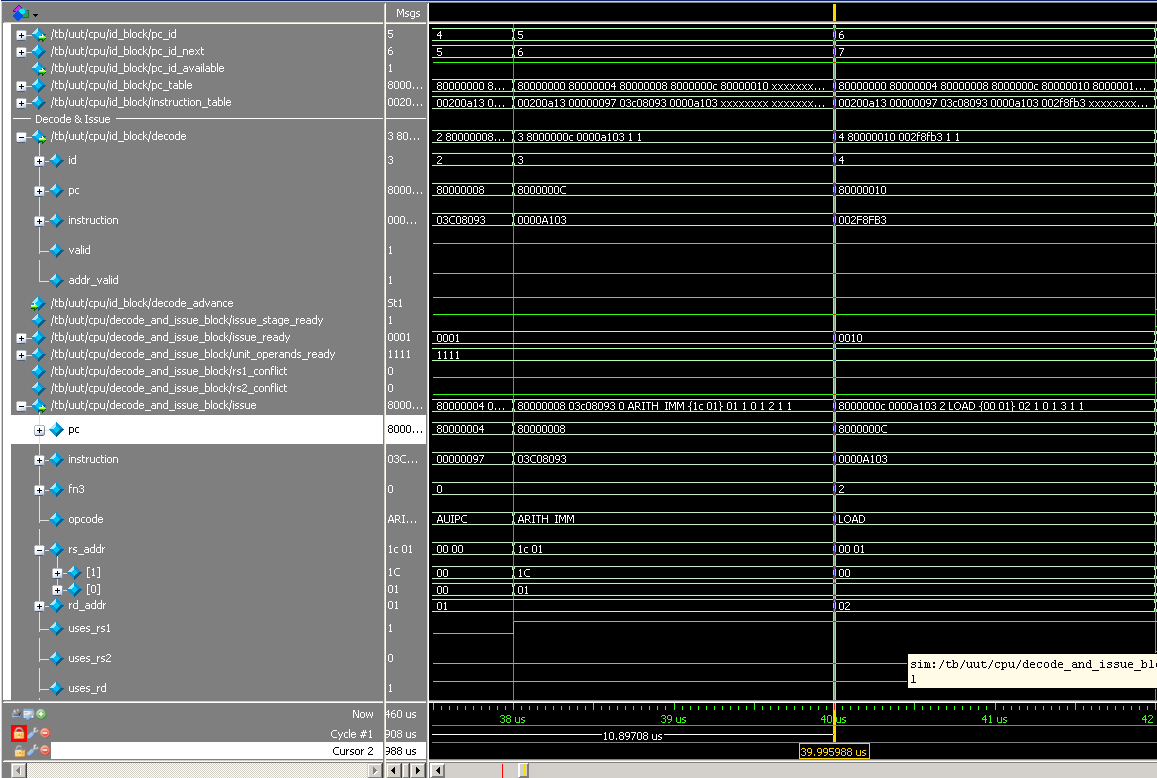
\includegraphics[height=0.42\textheight]{img/t3-modelsim}
	\caption{Скриншот запуска симуляция в среде Modelsim -- команды с адресом 8000000с на второй итерации.}
	\label{img:t3-modelsim}
\end{figure}

\section{Задание №4}

\subsection*{Условие задания}
Получить снимок экрана, содержащий временную диаграмму выполнения стадии выполнения команды с адресом 80000020 на первой итерации.

\subsection*{Результаты выполнения}

\begin{figure}[h]
	\centering
	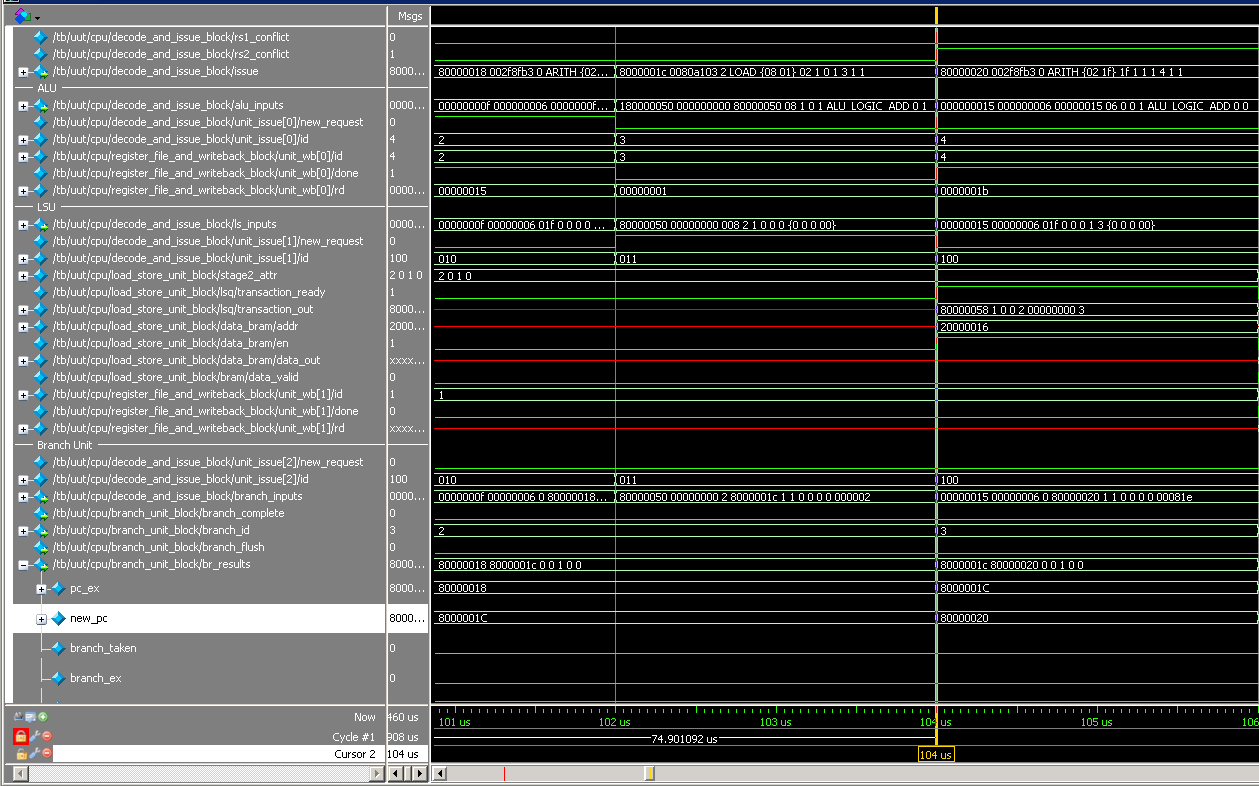
\includegraphics[height=0.42\textheight]{img/t4-modelsim}
	\caption{Скриншот запуска симуляция в среде Modelsim -- команды с адресом 80000020 на первой итерации.}
	\label{img:t4-modelsim}
\end{figure}

\section{Задание №5}

\subsection*{Условие задания}

В процесссе выполнения задания необходимо выполнить следующие действия:
\begin{enumerate}
	\item Исправить 76-ю строку файла $taiga/examples/zedboard/taiga_wrapper.sv$ так, чтобы там был указан путь к файлу $.hex$, соответствующему программе по индивидуальному варианту. Сохранить файл.
	\item Перекомпилировать исправленный файл. Для этого в окне программы Modelsim найти вкладку Library, в этой вкладке найти модуль work → taiga\_wrapper. В контекстном меню модуля выбрать пункт Recompile.
	\item Ввести в командой строке Modelsim команду $restart;$ $run$ $460us$ для перезапуска симуляции.
	\item Получить временную диаграмму сигналов выполнения программы индивидуального варианта.
	\item Сравнить значение регистра x31 (сигнал $/tb/register_file[31]$) на момент окончания выполнения программы с тем, который был получен в Задании №1.
	\item Получить снимок экрана, содержащий временные диаграммы сигналов, соответствующих всем стадиям выполнения команды, обозначенной в тексте программы символом \#!.
	\item Анализируя диаграмму заполнить трассу выполнения программы. Рекомендуется использовать для этого файл pipeline.ods, содержащий трассу тестового примера.
	\item Сделать вывод об эффективности выполнения программы и о путях оптимизации.
	\item Провести оптимизацию программы путем перестановки команд для устранения конфликтов.
	\item Перекомпилировать программу и перезапустить симуляцию.
	\item Заполнить трассу выполнения оптимизированной программы.
	\item Сравнить трассы выполнения неоптимизированной и оптимизированной версии, сделать выводы.
\end{enumerate}

\subsection*{Результаты выполнения}

\subsubsection*{Трасса работы программы}
Трасса работы представлена на рисунке \ref{img:t5-trasa-01}.

\begin{figure}[h]
	\centering
	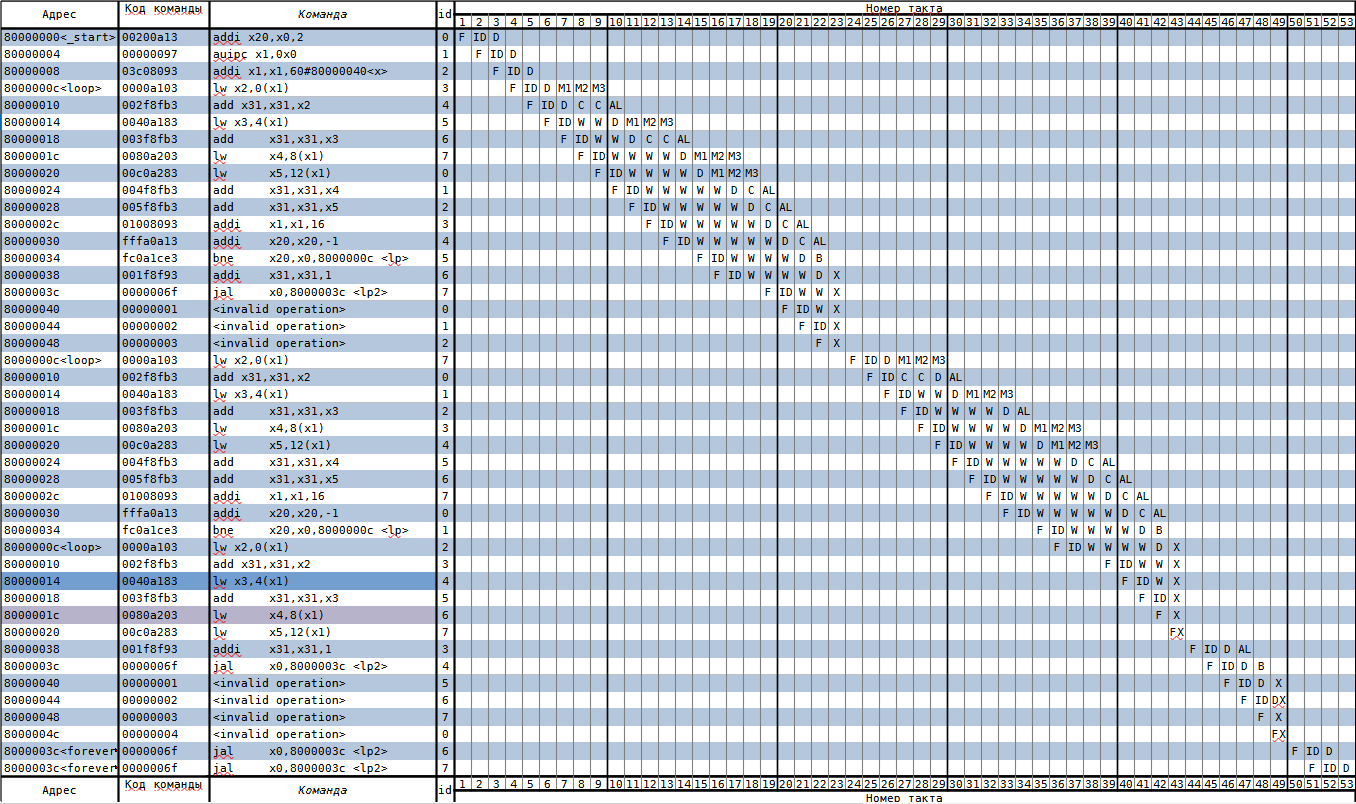
\includegraphics[height=0.4\textheight]{img/t5-trasa-01}
	\caption{Трасса работы программы.}
	\label{img:t5-trasa-01}
\end{figure}

\clearpage

\subsubsection*{Временные диаграммы}
Временные диаграммы сигналов, соответствующих всем стадиям выполнения команды, обозначенной в тексте программы символом \#! (add x31, x31, x2) представлены на рисунке \ref{img:t5-modelsim}.
\begin{figure}[h]
	\centering
	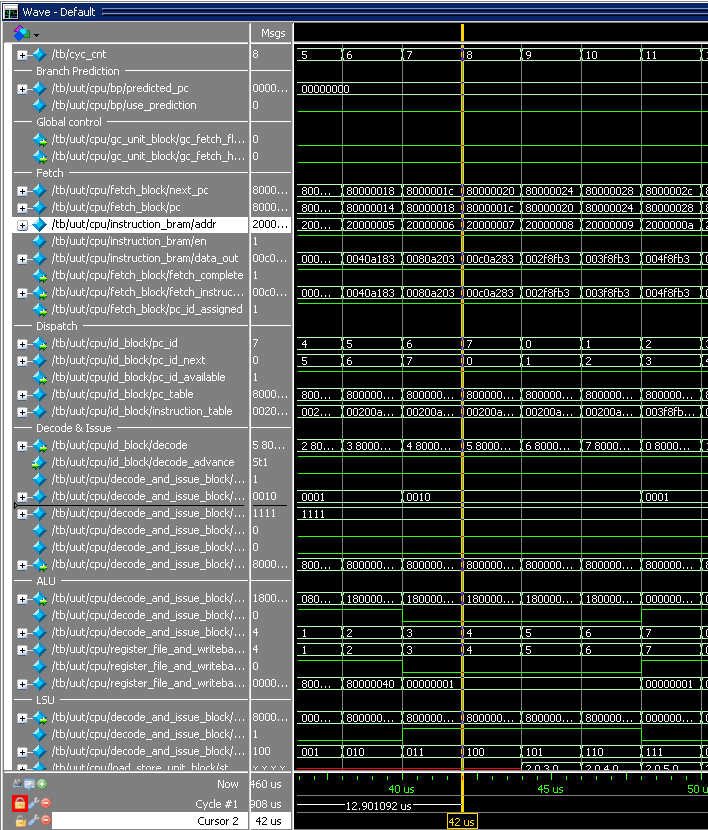
\includegraphics[height=0.6\textheight]{img/t5-modelsim}
	\caption{Временные диаграммы сигналов.}
	\label{img:t5-modelsim}
\end{figure}

\clearpage

\subsubsection*{Вывод и предложение по оптимизации}
Как видно на трассе работы программы, представленной на рисунке \ref{img:t5-modelsim}, конфликты возникают из-за того, что данные загружаются в память тогда, когда уже готова выполниться операция сложения тех данных, которые загружаются. Из-за этого и возникают конфликты, так как нечего складывать, так как в памяти пока нет ничего. 

Можно заметить, что трижды возникает ситуация ошибочной выборки, которая негативно сказывается на производительности, так как приводит к очистки конвейера.

Оптимизировать программы можно тем, что сначала загрузить все данные в память, а потом их складывать. Тем самым у нас не будет конфликтов, не будет ожидания конца загрузки данных в память.

В итоге, можно будет уменьшить программу на 2 такта 4 раза в программе, на 1 такт 3 раза в программе, то есть на 11/53 = 20\% программа будет работать быстрее.

\clearpage

\subsubsection*{Оптимизированная программа}

Код программы представлен в листинте \ref{lst:v111}

\begin{lstlisting}[label=lst:v111,caption=Код программы 9 варианта(оптимизированный)]
.section .text
.globl _start;
len = 8
enroll = 4 
elem_sz = 4 

_start:
addi x20, x0, len/enroll
la x1, _x
lp:
lw x2, 0(x1)
lw x3, 4(x1)
lw x4, 8(x1)
lw x5, 12(x1)
add x31, x31, x2 #!
add x31, x31, x3
add x31, x31, x4
add x31, x31, x5
addi x1, x1, elem_sz*enroll
addi x20, x20, -1
bne x20, x0, lp
addi x31, x31, 1
lp2: j lp2

.section .data
_x:     .4byte 0x1
.4byte 0x2
.4byte 0x3
.4byte 0x4
.4byte 0x5
.4byte 0x6
.4byte 0x7
.4byte 0x8
\end{lstlisting}

\clearpage

Дизассемблерный код представлен на листинге \ref{lst:v222}.

\begin{lstlisting}[label=lst:v222,caption=Дизассемблированный код 9 варинта (оптимизированный)]
Disassembly of section .text:

80000000 <_start>:
80000000:       00200a13        addi    x20,x0,2
80000004:       00000097        auipc   x1,0x0
80000008:       03c08093        addi    x1,x1,60 # 80000040 <_x>

8000000c <lp>:
8000000c:       0000a103        lw      x2,0(x1)
80000010:       0040a183        lw      x3,4(x1)
80000014:       0080a203        lw      x4,8(x1)
80000018:       00c0a283        lw      x5,12(x1)
8000001c:       002f8fb3        add     x31,x31,x2
80000020:       003f8fb3        add     x31,x31,x3
80000024:       004f8fb3        add     x31,x31,x4
80000028:       005f8fb3        add     x31,x31,x5
8000002c:       01008093        addi    x1,x1,16
80000030:       fffa0a13        addi    x20,x20,-1
80000034:       fc0a1ce3        bne     x20,x0,8000000c <lp>
80000038:       001f8f93        addi    x31,x31,1

8000003c <lp2>:
8000003c:       0000006f        jal     x0,8000003c <lp2>
\end{lstlisting}
\clearpage

Можно сказать, что данная программа эквивалентна следующему псевдокоду на языке C, представленному на листинге \ref{lst:v333}.

\begin{lstlisting}[label=lst:v333,caption=Псевдокод программы 9 варинта (оптимизированный)]
#define len 8
#define enroll 4
#define elem_sz 4
int _x[]={1,2,3,4,5,6,7,8};
void _start() {
	int x20 = len/enroll;
	int *x1 = _x;
	
	do {
		int x2 = x1[0];
		int x3 = x1[1];
		int x4 = x1[2];
		int x5 = x1[3];
		x31 += x2;
		x31 += x3;
		x31 += x4;
		x31 += x5;
		x1 += enroll;
		x20--;
	} while(x20 != 0);
	x31++;
	while(1){}
}
\end{lstlisting}

\clearpage

\subsubsection*{Трасса работы оптимизированной программы}
Трасса работы представлена на рисунке \ref{img:t5-trasa-02}.

\begin{figure}[h]
	\centering
	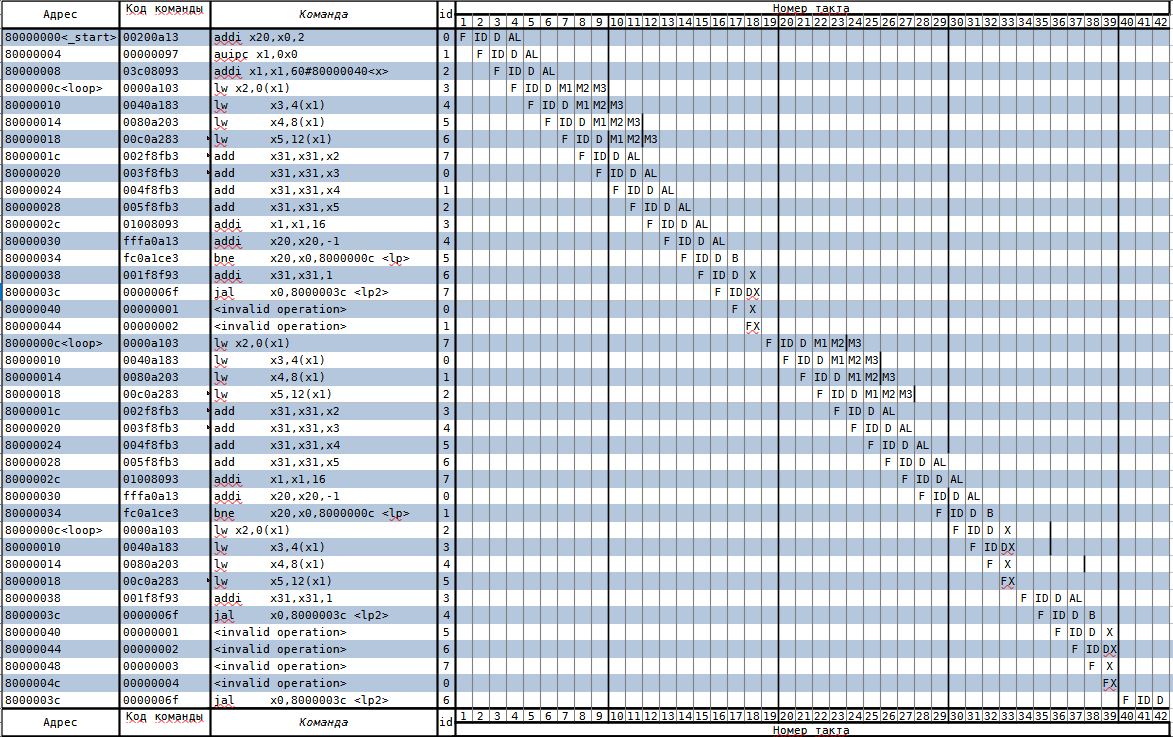
\includegraphics[height=0.4\textheight]{img/t5-trasa-02}
	\caption{Трасса работы оптимизированной программы.}
	\label{img:t5-trasa-02}
\end{figure}

